
\section{Background}
\label{sec:background}
Given that this is our first project for this class, we decided to stick mostly to models that had been mentioned in class. As such, we tried out the linear regression, stochastic gradient descent (SGD), ridge regression, and LASSO models from the Python \texttt{scikit-learn} library. We also tried a stochastic gradient descent classification model, \texttt{SGDClassifier}, from the same library as well.
\begin{itemize}
    \item \textbf{Linear regression} - A straightforward model that focuses on finding the weights associated with the least cost in a linear combination of the features of the dataset. 
    \item \textbf{SGD} - Similar to linear regression, except the entire set of training examples is not evaluated each time a decision about minimizing the cost function is made. Instead, a random training example is chosen, and the minimum point of the cost function is calculated using that randomly chosen training example.
    \item \textbf{Ridge regression} - A version of linear regression that employs an L-2 regularization strategy. Ridge regression regulates the complexity of the curve used to fit the data by employing a penalty for higher weights. The specific penalty used is called the L-2 penalty and is defined as $$\sum_{j=1}^{n} \theta_{j}^{2}$$.
    \item \textbf{LASSO} - Similar to ridge regression, except the regularization penalty used is L-1, which is defined as $$\sum_{j=1}^{n} |\theta_{j}|$$.
    \item \textbf{SGDClassifier} - While this model was not talked about in class, it is similar to the regular SGD model in that gradient descent updates are made using single or batches of training examples instead of the whole dataset. However, a major difference is that \texttt{SGDClassifier} is used for classification problems. A classification problem is any problem where the target variable can only take on a finite set of discrete values. Since our target variable, quality, can only take on values from 0 to 10 (inclusive), this problem can also be considered as a classification problem. \texttt{SGDClassifier} also makes use of a regularization penalty.
\end{itemize}
Before any of these models could be run, however, it was necessary that the data went through some preprocessing. We used the \texttt{pandas} Python library to import the data from the files and store them with the appropriate column headers. We used one file to house all the functions needed to preprocess the data, which we called \path{winequality.py}. This file held the following functions: \path{read_file}, \path{select_features}, \path{make_poly}, \path{standardize}, \path{drop_outliers}, \path{split}, \path{get_XY}, and \path{get_preprocessed_dataset}.
\begin{enumerate}
    \item The \path{read_file} function was used to read in the .csv file and store it in a DataFrame object.
    \item Then, we split the file into the features and the quality, since we only wanted to apply some preprocessing functions to the features dataset.
    \item The \path{select_features} function was used to trim down the dataset to only the features we wanted to train the models with. The way we decided which features to use will be explained shortly.
    \item The \path{make_poly} function used \texttt{PolynomialFeatures} imported from the \texttt{scikit-learn} library. We used \texttt{PolynomialFeatures} to add extra columns to the dataset to simulate higher-order polynomials.
    \item The \path{standardize} function was then used to standardize the dataset using \textt{StandardScaler} from the \texttt{scikit-learn} library.
    \item The standardized DataFrame had the quality variable added back in before we dropped the outliers from the dataset. The \path{drop_outliers} function dropped any outliers that weren't within $3$ standard deviations of the mean of any column.
    \item The \path{split} function split the dataset into a 60\%-20\%-20\% split to represent the training, validation, and testing datasets.
\end{enumerate}      
The \path{get_XY} function accepted a DataFrame as input and returned the features and the target separately. Finally, \path{get_preprocessed_dataset} was a master function that called all of the other functions and returned the preprocessed dataset.\\

To begin the process of feature selection, we ran some statistical analyses on our datasets. First, we created graphs of quality scores vs. each feature to see if there were any outliers. A few of these graphs can be seen in Figures 1, 2, and 3. All feature data came from the original dataset, prior to standardization, which is why the graphs have different scales. A few of the graphs showed some data points that were considerably different from any others. For example, the citric acid value for entry $152$ of the red wine dataset was $3.7$ standard deviations above the mean for citric acid. Even a single outlier can have a significant effect on the relationship between two variables \cite{aia}. Keeping this in mind, we decided to drop all outliers from our datasets.\\
\begin{figure}[htb]

  \centering  % centers the image in the column

  % replace the second argument below with your filename. I like to
  % place all my figures in a sub-directory to keep things organized
  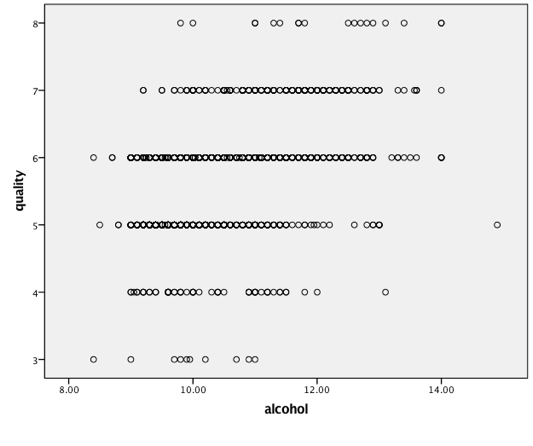
\includegraphics[width=0.42\textwidth]{1.png}

  % *Every* figure should have a descriptive caption.
  \caption{Correlation Between Alcohol and Quality for Red Wine}

  % The label is a handle you create so that you can refer to this
  % figure (using the \ref{} command) from other parts of your
  % document. LaTeX automatically renumbers figures and updates
  % references when you recompile, so you should do it this way rather
  % than hard-coding in references. Notice that I've also been
  % creating labels for the various sections in the document; I could
  % use \ref{} command to refer to those sections using their labels
  % too.
  \label{fig:tex}

  \end{figure}
  
  \begin{figure}[htb]

  \centering  % centers the image in the column

  % replace the second argument below with your filename. I like to
  % place all my figures in a sub-directory to keep things organized
  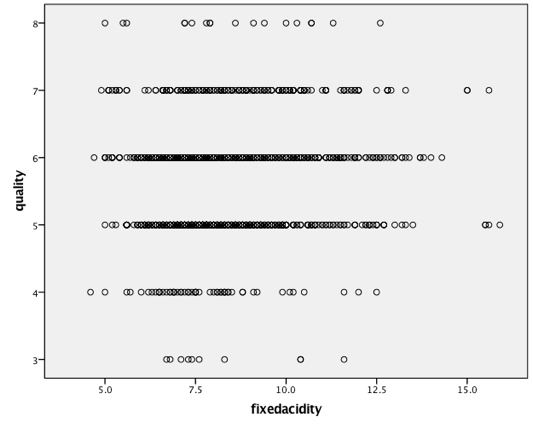
\includegraphics[width=0.42\textwidth]{2.png}

  % *Every* figure should have a descriptive caption.
  \caption{Correlation Between Fixed Acidity and Quality for Red Wine}

  % The label is a handle you create so that you can refer to this
  % figure (using the \ref{} command) from other parts of your
  % document. LaTeX automatically renumbers figures and updates
  % references when you recompile, so you should do it this way rather
  % than hard-coding in references. Notice that I've also been
  % creating labels for the various sections in the document; I could
  % use \ref{} command to refer to those sections using their labels
  % too.
  \label{fig:tex}

  \end{figure}
   \begin{figure}[htb]

  \centering  % centers the image in the column

  % replace the second argument below with your filename. I like to
  % place all my figures in a sub-directory to keep things organized
  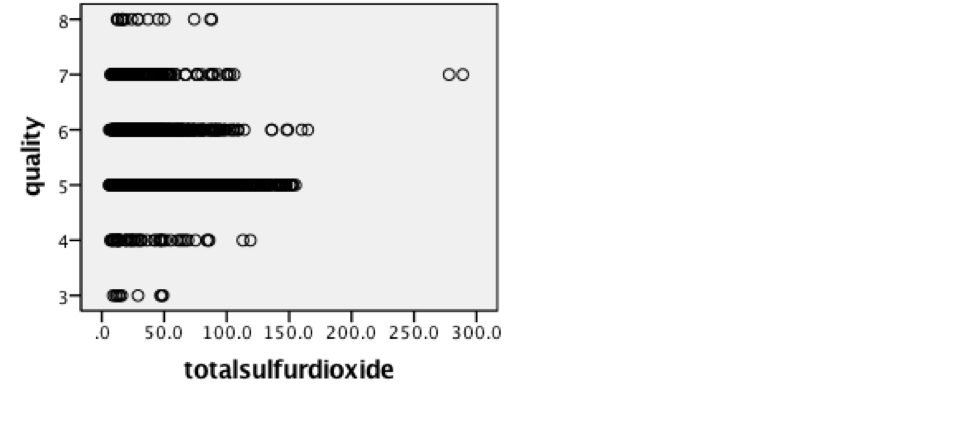
\includegraphics[width=0.42\textwidth]{3.png}

  % *Every* figure should have a descriptive caption.
  \caption{Correlation Between Total Sulfur Dioxide and Quality for Red Wine}

  % The label is a handle you create so that you can refer to this
  % figure (using the \ref{} command) from other parts of your
  % document. LaTeX automatically renumbers figures and updates
  % references when you recompile, so you should do it this way rather
  % than hard-coding in references. Notice that I've also been
  % creating labels for the various sections in the document; I could
  % use \ref{} command to refer to those sections using their labels
  % too.
  \label{fig:tex}

  \end{figure}
  
\newpage

Next, we computed a Pearson's correlation coefficient between each feature and quality for each dataset. Figures 4 and 5 contain the correlation coefficients we computed, ordered from the strongest to the weakest. We discovered that pH, free sulfur dioxide, and residual sugar showed the weakest correlations with quality for the red wine dataset. Sulphates, citric acid, and free sulfur dioxide showed the weakest correlations with quality for the white wine dataset. Given these results, we ran some experiments excluding some of these features that were weakly correlated with quality. A summary of our experiments and results is provided in the next two sections.
\begin{figure}[htb]
  \centering % centers the entire table

  % The following line sets the parameters of the table: we'll have
  % three columns (one per 'c'), each
  % column will be centered (hence the 'c'; 'l' or 'r' will left or
  % right justify the column) and the columns
  % will have lines between them (that's the purpose of the |s between
  % the 'c's).
 \begin{tabular}{|c|c|} 
   \hline \hline % draws two horizontal lines at the top of the table
    Feature & Correlation with Quality \\ % separate column contents using the &
    \hline % line after the column headers
    Alcohol & $0.476$** \\
     \hline
    Volatile Acidity & $-0.391$** \\
     \hline
    Sulphates & $0.251$** \\
     \hline
    Citric Acid   & $0.226$** \\
     \hline
    Total Sulfur Dioxide  & $-0.185$** \\
     \hline
    Density  & $-0.175$** \\
     \hline
    Chlorides & $-0.129$** \\
     \hline
    Fixed Acidity  & $0.124$** \\
     \hline
    pH  & $-0.058$* \\
     \hline
    Free Sulfur Dioxide    & $0.051$* \\
     \hline
    Residual Sugar   & $0.014$ \\
  
    \hline \hline  
    \end{tabular}
  % As with figures, *every* table should have a descriptive caption
  % and a label for ease of reference.
  \caption{Table of Feature Correlation with Quality for Red Wine.}
  \floatfoot{** indicates the correlation is significant at the 0.01 level, while * indicates the correlation is significant at the 0.05 level.}
  \label{tab:example}

\end{figure}

  \begin{figure}[htb]
  \centering % centers the entire table

  % The following line sets the parameters of the table: we'll have
  % three columns (one per 'c'), each
  % column will be centered (hence the 'c'; 'l' or 'r' will left or
  % right justify the column) and the columns
  % will have lines between them (that's the purpose of the |s between
  % the 'c's).
 \begin{tabular}{|c|c|} 
   \hline \hline % draws two horizontal lines at the top of the table
    Feature & Correlation with Quality \\ % separate column contents using the &
    \hline % line after the column headers
    Alcohol & $0.436$** \\
     \hline
    Density & $-0.307$** \\
     \hline
    Chlorides & $-0.210$** \\
     \hline
    Volatile Acidity   & $-0.195$** \\
     \hline
    Total Sulfur Dioxide  & $-0.175$** \\
     \hline
    Fixed Acidity  & $-0.114$** \\
     \hline
    pH & $0.099$** \\
     \hline
    Residual Sugar & $-0.098$** \\
     \hline
    Sulphates  & $0.054$** \\
     \hline
    Citric acid   & $-0.009$ \\
     \hline
    Free Sulfur Dioxide  & $0.008$ \\
  
    \hline \hline  
    \end{tabular}
  % As with figures, *every* table should have a descriptive caption
  % and a label for ease of reference.
  \caption{Table of Feature Correlation with Quality for White Wine}
  \floatfoot{** indicates the correlation is significant at the 0.01 level, while * indicates the correlation is significant at the 0.05 level.}
  \label{tab:example}


\end{figure}


